\documentclass[10pt,journal,compsoc]{IEEEtran}
%
% *** CITATION PACKAGES ***
%
\ifCLASSOPTIONcompsoc
  % IEEE Computer Society needs nocompress option
  % requires cite.sty v4.0 or later (November 2003)
  \usepackage[nocompress]{cite}
\else
  % normal IEEE
  \usepackage{cite}
\fi
% cite.sty was written by Donald Arseneau

% *** GRAPHICS RELATED PACKAGES ***
%
\ifCLASSINFOpdf
  \usepackage[pdftex]{graphicx}
  % declare the path(s) where your graphic files are
  % \graphicspath{{../pdf/}{../jpeg/}}
  % and their extensions so you won't have to specify these with
  % every instance of \includegraphics
  % \DeclareGraphicsExtensions{.pdf,.jpeg,.png}
\else
  % or other class option (dvipsone, dvipdf, if not using dvips). graphicx
  % will default to the driver specified in the system graphics.cfg if no
  % driver is specified.
  % \usepackage[dvips]{graphicx}
  % declare the path(s) where your graphic files are
  % \graphicspath{{../eps/}}
  % and their extensions so you won't have to specify these with
  % every instance of \includegraphics
  % \DeclareGraphicsExtensions{.eps}
\fi

\usepackage{listings}

% *** PDF, URL AND HYPERLINK PACKAGES ***
%
\usepackage{hyperref}


\begin{document}

\title{Staged computation: the technique you didn't know you were using}

\author{Konrad Hinsen}

% The paper headers
\markboth{Computing in Science and Engineering}%
{Scientific Programming department}
% The only time the second header will appear is for the odd numbered pages
% after the title page when using the twoside option.
% 
\maketitle

A quick Web search for ``staged computation'' will convince you that it refers to an exotic technique of interest mainly to programming language designers and implementers. Nothing could be further from the truth. It's a technique that everybody is using all the time, and it's one of the main reasons why reproducible results are so difficult to achieve. In other words, it's something that every computational scientist should know about.

\vspace{3mm}

By definition, a staged computation is a computation that proceeds as a sequence of multiple stages, in which each stage produces the \textit{code} for the next stage, except for the last stage that produces the final result. Most of the references you will find in a Web search are about so-called meta-programming techniques, in which a program's source code is transformed before actually being compiled into an executable. The most widely used meta-programming technique in scientific computing is the use of macros in the C and C++ languages. These macros are rules for rewriting the source code before compilation that are used for specializing the code, or for adapting it different platforms. Other languages have more elaborate metaprogramming tools, in particular the languages of the Lisp family.

However, the kind of staged computation that I will discuss here is something quite different: it is the very use of compilers. A compiler transforms a program from one notation (``source code'') to another notation (``executable binary''). Executing a piece of source code thus requires two stages: the first stage, compilation, produces the code that is run in the second stage, execution. But that is not the end of the story. The compiler you run is typically an executable binary stored somewhere in your computer's file system, and so are the libraries that a program makes use of. These binaries have been produced by someone else, on another computer, using yet another compiler. So our two-stage computation is really a many-stage computation, with the results of the initial stages stored on some server for downloading by people like you. Package managers, such as \texttt{apt} used by Linux distributions such as Debian or Ubuntu, or \texttt{Homebrew} for macOS, make this approach straightforward in practice.

\section{Multi-stage reproducibility}

\begin{figure}[tbh]
\centering
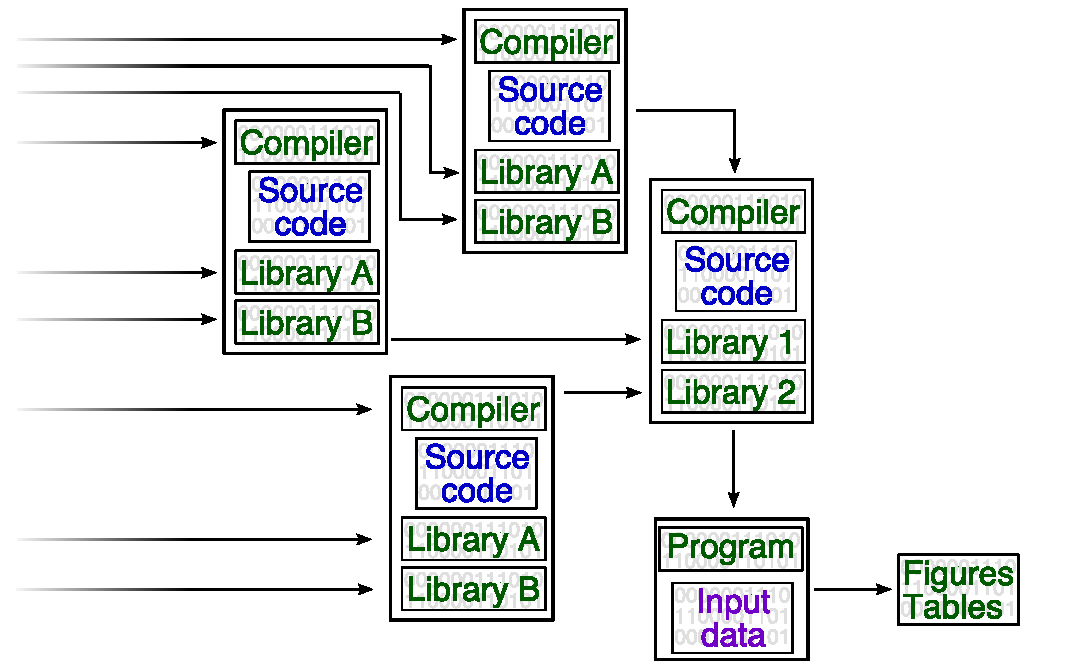
\includegraphics[width=3.5in]{fig-1.pdf}
\caption{The final stages of a typical staged computation. Items shown in blue are human input. Items shown in magenta are other input, typically from experiments. Items shown in green are the output of a computation.}
\label{fig:staged-computation}
\end{figure}

Fig.~\ref{fig:staged-computation} provides a visual illustration of a staged computation. Each box in this diagram corresponds to data stored in a file, but there are three distinct categories of data. The first category, shown in blue, is input authored by humans, i.e. mostly program source code. The second category, shown in magenta, is observational input, typically coming from experimental equipment. The third and dominant category, shown in green, is results of computations. The computations that produce them are indicated by arrows that link inputs to outputs.

What we would like to be reproducible is the box in the bottom right, i.e. the figures and tables we put into our publications. The important message of Fig.~\ref{fig:staged-computation} is that \textit{reproducing these results requires all the other items in the diagram to be precisely identified and either archived or themselves reproducible.} And since even a modest computation can accumulate hundreds of little boxes, this is not a trivial requirement.

Let's look at what this means for our three categories of items. Human input is the easiest case: it cannot be reproduced, so it must be archived. Note that ``archiving'' means more than just storing a copy in a safe place. That would be a backup, not an archival copy. Archiving requires producing a safely guarded copy plus a handle via which this copy can be retrieved unambiguously. That handle could be a file name or a URL (both very fragile), a Digital Object Identifier (DOI), which is already more robust, or ideally a handle computed from the content itself \cite{content-addressable}, such as the identifiers used by Software Heritage \cite{SWHid}. Since human input tends to evolve in the course of a research project, it is also advisable to keep it under version control \cite{version-control}. Both  Zenodo (https://zenodo.org/) and Software Heritage (https://www.softwareheritage.org/) provide facilities for easily archiving version-controlled human input.

It is more difficult to give general recommendations for observational input, because that is a very diverse category. Like human-authored input, observational input is not reproducible, and must therefore be archived. For choosing an adequate archiving technique and platform, the nature and size of the data matters, but also legal criteria such as ownership or privacy.

For the computed results, in particular compiled software, we have the choice between archiving and reproducing. Unfortunately, the tools we have been using for decades to manage software support neither option satisfactorily. They have been designed for installing, updating, and deploying software, but not for tracking provenance or reproducing earlier states. These tasks must therefore be assumed by humans, who are not very good at managing hundreds of items. This is why reproducible computations remain such a tough challenge. The good news is that computers are very good at dealing with large problems, meaning that we can delegate the management of staged computations to software tools, as I will show later.

\begin{figure*}[!t]
\begin{lstlisting}[
  language=C,
  basicstyle=\small,
]
#include <math.h>
#include <stdio.h>

int main()
{
    printf( "M_PI                         : %.10lf\n", M_PI);
    printf( "4 * atan(1.)                 : %.10lf\n", 4.*atan(1.));
    printf( "Leibniz' formula (four terms): %.10lf\n", 4.*(1.-1./3.+1./5.-1./7.));
    return 0;
}
\end{lstlisting}
\caption{A very simple computation in C.}
\label{lst:pi}
\end{figure*}

\section{The state of the art}

Consider the very simple program shown in Fig.~\ref{lst:pi}, which does a few computations and prints the results. On a typical Linux system, you would run it using
\begin{verbatim}
gcc pi.c -o pi
./pi
\end{verbatim}
assuming you are using the popular GNU Compiler Collection. The few lines of text printed by the program are the final result. That's what goes into the bottom-right box in Fig.~\ref{fig:staged-computation}. The executable binary \texttt{pi} is the ``Program'' in the box on the left end of the arrow. There is no ``Input data'' in this case. The source code file \texttt{pi.c} is the ``Source code'' in the box above. The ``Compiler'' is \texttt{gcc}. And it looks like we have no libraries, so we have properly identified everything in the rightmost three boxes of Fig.~\ref{fig:staged-computation}. That's a good start!

The bad news is that appearances are deceptive: we do have libraries, the compiler is merely hiding them from us. Under the hood, the compiler runs additional programs such as \texttt{as} or \texttt{collect2}, and adds libraries from the C language runtime system. We need to add this hidden stuff, with version numbers, to the ``Compiler'' and ``Library'' fields of the box. And with compilers playing hide-and-seek, we need a more reliable way to figure out all of our dependencies!

I suspect that many readers think that I am exaggerating. We are talking about a minuscule C program. All it takes to run it is a toolchain for compiling C programs. It doesn't matter if I use version~7 or version~9 of \texttt{gcc}. It matters even less what the version number of \texttt{collect2} is, whatever it may do. And all the stages before the compilation of \texttt{pi.c} shouldn't matter at all. If the \texttt{gcc} that I am running has passed its test suite, all should be fine.

This reasoning is, in fact, correct most of the time, when applied to C compilers and other stable tools and libraries. But most of the time is not all of the time. One particular subtle point is floating-point arithmetic, which has the reputation of being fundamentally irreproducible \cite{approximation-tower}. And yet, at the level of the operations defined by the standard IEEE-754 (which all processors and compilers today respect), floating-point arithmetic is perfectly deterministic. The problem is that programmers don't write their code in terms of IEEE-754 operations. The C language doesn't even give access to that level. It's the compiler that generates those low-level instructions, and it assumes that the programmer doesn't care about the differences due to round-off. So if you want reproducible floating-point results, their full specification is your code plus the C compiler plus the compilation options.

More importantly, the ``details don't matter'' reasoning fails for large software assemblies, in which pieces you have never heard about but which have an impact on the final results may change because of bugs or voluntary decisions to break backwards compatibility. Under the Guix package manager, about which I will say more below, running the C program in Fig.~\ref{lst:pi} requires four packages (gcc, binutils, glibc, ld-wrapper, the last one being a Guix-specific package). That's what takes the green-colored slots in the rightmost ``Compiler'' box in Fig.~\ref{fig:staged-computation}. For a Python script using the popular NumPy and SciPy extensions, that's already 24 packages. If you include all the packages from the earlier stages of the computation, you get 89~packages for a C program, but 501 for Python + NumPy + SciPy. Figuring out which of these packages should be irrelevant details becomes a serious challenge.

Let's move on for now, assuming that we can somehow keep track of hundreds of dependencies. We must then either archive the compiled code, or make it reproducible. But we can immediately eliminate ``archiving'' because there is no practically usable infrastructure for this. Sure, package managers download compiled code from servers, but these servers are \textit{caches}, designed for increasing the efficiency of software distribution. They are not archives from which binaries could be retrieved at arbitrary later times via an unambiguous handle. That also applies to services such as DockerHub that hold container images.

The situation looks more promising for making all compiled code reproducible. Package managers are based on build recipes, which is the code that is run to re-build the package. Likewise, containers are usually built from such recipes, e.g. the well-known Dockerfiles. Unfortunately, a closer look reveals that most of these build recipes are not reproducible. They say something like ``download the current Python source code and compile it with the current version of gcc.'' That's great for regularly updating software, which is after all what package and container managers were designed for, but it's not reproducible.

\section{Guix to the rescue}

The Guix package manager (http://guix.gnu.org/) for GNU/Linux was designed from the start with reproducibility in mind, and offers the best support for reproducible research that is currently available. More specifically, it is based on two fundamental concepts:
\begin{itemize}
\item An explicit representation of the full staged computation graph of Fig.~\ref{fig:staged-computation}, for all software packages, containing all information that can potentially impact results, and referring to specific versions of all source code.
\item Execution in restricted environments. Guix can run programs in environments where only explicitly listed software is available, providing a guarantee that the programs have no other dependencies. These restricted environments are used for building software packages, but are also available to users for running their own code.
\end{itemize}

To run the example from Fig.~\ref{lst:pi} in a restricted environment in Guix, I would type
\begin{verbatim}
$ guix environment --container \
                   --ad-hoc gcc-toolchain
[env]$ gcc pi.c -o pi
[env]$ ./pi
\end{verbatim}
The first line creates a restricted environment with access to a single software package (\texttt{gcc-toolchain}), a single directory (the current one), and no network access at all. It then starts a shell in that environment, into which the following two lines are typed. The option \texttt{--container} provides the strongest possible isolation of that environment, but less restrictive versions are also available. The fact that my program works correctly in that environment proves that it has no dependencies other than \texttt{gcc-toolchain}, which is a package specifically designed for C programming and contains the \texttt{gcc} compiler plus the utilities and libraries it requires to function. 
To make computations in such environments reproducible, all I need to do is note the exact version of Guix that I am using:
\begin{verbatim}
$ guix describe -f recutils
name: guix
url: https://git.savannah.gnu.org/git/guix.git
commit: 769b96b62e8c09b078f73adc09fb860505920f8f
\end{verbatim}
The Guix version is given by the \texttt{commit} field, which is a unique and persistent handle. I can then at any time in the future reproduce the environment, and thus my computation:
\begin{verbatim}
$ guix time-machine \
       --commit=769b96b62e8c09b078f73adc \
       -- \
       environment --container \
                   --ad-hoc gcc-toolchain
[env]$ gcc pi.c -o pi
[env]$ ./pi
\end{verbatim}
If you think that the first line is rather long, consider that it replaces a whole Docker container!

Like other package managers, Guix downloads pre-compiled binary versions of its packages from a caching server if available. Otherwise, or upon explicit user request, Guix recompiles everything from source code. Well, almost everything: a minimal archived core package called the bootstrap seed is always downloaded in binary form. It contains a basic compiler that is used to get the staged computations started. You can't avoid having to download that bootstrap seed in binary form, but if you are particularly paranoid, you can then recompile it yourself, and verify that you get the same files, bit for bit.

Since Guix stores the complete staged computation graph, you can also explore it using Guix' command line tools for standard tasks such as querying the version numbers of the packages. For more advanced needs, you can write scripts in Guile, the dialect of Scheme that Guix is written in. This is what I did to obtain the dependency counts that I quoted earlier. For readers interested in the technical details, there is a post on the Guix blog \cite{guix-blog}.

At this time, Guix is still a tool for early adopters. Its package collection is not nearly as complete as those of well established distributions, and its tools still evolve rather rapidly. However, it shows that reproducible staged computations are possible, and it is actually already very usable in practice if all the software you need is in there. Check it out for yourself!

% references section

% can use a bibliography generated by BibTeX as a .bbl file
% BibTeX documentation can be easily obtained at:
% http://mirror.ctan.org/biblio/bibtex/contrib/doc/
% The IEEEtran BibTeX style support page is at:
% http://www.michaelshell.org/tex/ieeetran/bibtex/
%\bibliographystyle{IEEEtran}
% argument is your BibTeX string definitions and bibliography database(s)
%\bibliography{IEEEabrv,../bib/paper}
%
% <OR> manually copy in the resultant .bbl file
% set second argument of \begin to the number of references
% (used to reserve space for the reference number labels box)

\begin{thebibliography}{1}

\bibitem{content-addressable}
K.~Hinsen,
\textit{The magic of content-addressable storage},
Computing in Science \& Engineering, early access,
DOI: 10.1109/MCSE.2019.2949441

\bibitem{SWHid}
R.~Di~Cosmo, M.~Gruenpeter, and S.~Zacchiroli,
\textit{Identifiers for Digital Objects: The Case of Software Source Code Preservation},
iPRES 2018 - 15th International Conference on Digital Preservation, Sep 2018, Boston, United States.
\href{http://doi.org/10.17605/OSF.IO/KDE56}{DOI:10.17605/OSF.IO/KDE56}

\bibitem{version-control}
K.~Hinsen, K.~L\"{a}ufer, G.K.~Thiruvathukal,
\textit{Essential Tools: Version Control Systems},
Computing in Science \& Engineering \textbf{11}, 81--91 (2009)

\bibitem{approximation-tower}
K.~Hinsen,
\textit{The approximation tower in computational science: why testing scientific software is difficult},
Computing in Science \& Engineering \textbf{17}, 72 (2015)

\bibitem{trusting-trust}
K.~Thompson,
\textit{Reflections on trusting trust},
Communications of the ACM \textbf{27}, 761 (1984)

\bibitem{guix-blog}
K.~Hinsen,
\textit{Reproducible computations with Guix},
\href{https://guix.gnu.org/blog/2020/reproducible-computations-with-guix/}{https://guix.gnu.org/blog/2020/reproducible-computations-with-guix/},
published January 14, 2020

\end{thebibliography}

% biography section

\begin{IEEEbiographynophoto}{Konrad Hinsen}
is a researcher at the Centre de Biophysique Mol\'{e}culaire in Orl\'{e}ans and at the Synchrotron SOLEIL in Saint Aubin. His research interests include protein structure and dynamics and scientific computing. Hinsen has a PhD in theoretical physics from RWTH Aachen University. Contact him at konrad.hinsen@cnrs.fr.
\end{IEEEbiographynophoto}

\end{document}
